\documentclass[10pt,t]{beamer} \usepackage[utf8]{inputenc}
\usepackage[T1]{fontenc} \usepackage{graphicx} \usepackage{grffile}
\usepackage{longtable} \usepackage{wrapfig} \usepackage{rotating}
\usepackage[normalem]{ulem} \usepackage{amsmath} \usepackage{textcomp}
\usepackage{amssymb} \usepackage{capt-of} \usepackage{hyperref}
\usepackage{relsize}
\input beamer_setup

% \usetheme{metropolis} \addtobeamertemplate{section
% page}{\let\insertsectionhead\insertsection}{} \usetheme{Frankfurt}
\usetheme{default}

% \metroset{titleformat title=allcaps}

\newcommand{\cris}{\textsf{CrIS}\xspace}
\newcommand{\airs}{\textsf{AIRS}\xspace}
\newcommand{\iasi}{\textsf{IASI}\xspace}

\newcommand{\twocolmod}[4] {
  \begin{columns}[T]
    \begin{column}[c]{#1\textwidth}
      {#3}
    \end{column}
    \begin{column}[c]{#2\textwidth}
      {#4}
    \end{column}
  \end{columns}
}

\newcommand{\threecol}[9] {
  \begin{columns}
    \begin{column}[#1]{#4\textwidth}
      \begin{center}
        {\small #7}
      \end{center}
    \end{column}
    \begin{column}[#2]{#5\textwidth}
      \begin{center}
        {\small #8}
      \end{center}
    \end{column}
    \begin{column}[#3]{#6\textwidth}
      \begin{center}
        {\small #9}
      \end{center}
    \end{column}
  \end{columns}
}

\newcommand{\fourcol}[8] {
  \begin{columns}
    \begin{column}[T]{#1\textwidth}
      \begin{center}
        {\small #5}
      \end{center}
    \end{column}
    \begin{column}[T]{#2\textwidth}
      \begin{center}
        {\small #6}
      \end{center}
    \end{column}
    \begin{column}[T]{#3\textwidth}
      \begin{center}
        {\small #7}
      \end{center}
    \end{column}
    \begin{column}[T]{#4\textwidth}
      \begin{center}
        {\small #8}
      \end{center}
    \end{column}
  \end{columns}
}

\newcommand{\twocolhead}[6] {
  \begin{columns}
    \begin{column}[#1]{#3\textwidth}
      \begin{center}
        {#5}
      \end{center}
    \end{column}
    \begin{column}[#2]{#4\textwidth}
      \begin{center}
        {#6}
      \end{center}
    \end{column}
  \end{columns}
}

\newcommand{\twocolc}[6] {
  \begin{columns}
    \begin{column}[#1]{#3\textwidth}
      \begin{center}
        {\small #5}
      \end{center}
    \end{column}
    \begin{column}[#2]{#4\textwidth}
      \begin{center}
        {\small #6}
      \end{center}
    \end{column}
  \end{columns}ur }

% ---------------------------------------------------------------------
\title[]{Using AIRS:CrIS SNOs to compare SDR product with and without \\
Polarization Correction}
  \author{C. Hepplewhite, L. Strow}
% ---------------------------------------------------------------------
% ---------------------------------------------------------------------
\begin{document}

% ---------------------------------------------------------------------
% ---------------------------------------------------------------------
\begin{frame}
  \titlepage
\end{frame}
% ---------------------------------------------------------------------
% ---------------------------------------------------------------------
\begin{frame}
  \frametitle{Overview}

  \begin{itemize}
  \item Use closely matched observations between \airs and J1-\cris to
    determine differences due to polarization correction applied to \cris.
  \item NOAA ADL SDR data are available for period December 2018 to January
    2019 (2 months), with and without polarization correction applied.
  \item \airs L1C data are available for the same time period.
  \item Simultaneuous near over-pass observational pairs are obtained with
    seprations between \airs and \cris FOVs of less than 10 minutes and 8 km.
  \item SNOs for \airs FOVs 43:48 and \cris FORs 15 and 16 are used.
  \item Approx. 242,000 SNO pairs are obtained.
  \end{itemize}

\end{frame}
% ---------------------------------------------------------------------
\begin{frame}
  \frametitle{Distribution Map}
  \begin{center}
    \noindent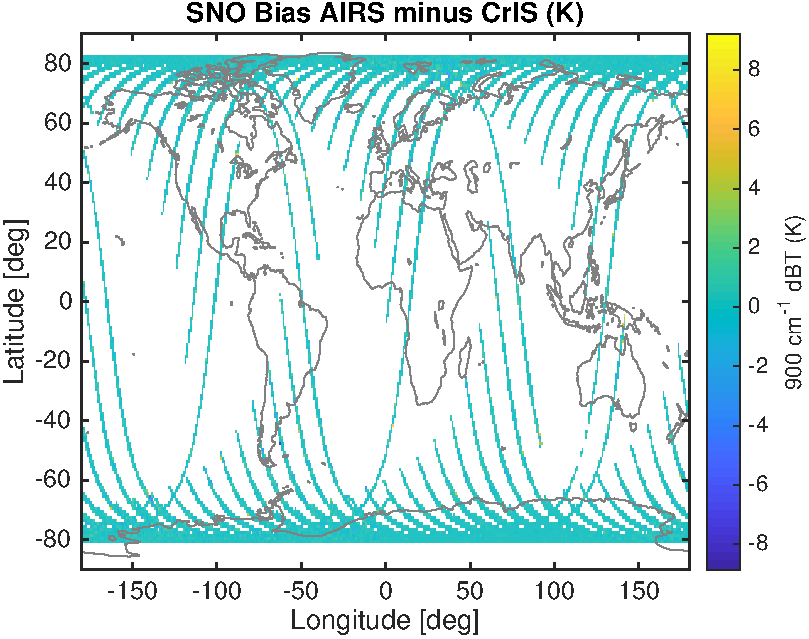
\includegraphics[width=0.75\textwidth]{Figs/sno_airs_cris2_bias_map.pdf}
  \end{center}
\end{frame}

% ---------------------------------------------------------------------
\begin{frame}
  \frametitle{Magnitude of the polarization correction}
  \vspace{-0.125in} %\relscale{0.95}
  \begin{itemize}
     \item Using AIRS as the transfer standard, take the double difference:
     \textit{ (\airs minus \cris with correction) minus (\airs minus \cris
      without correction}
  \end{itemize}
  
  \begin{center}
    \noindent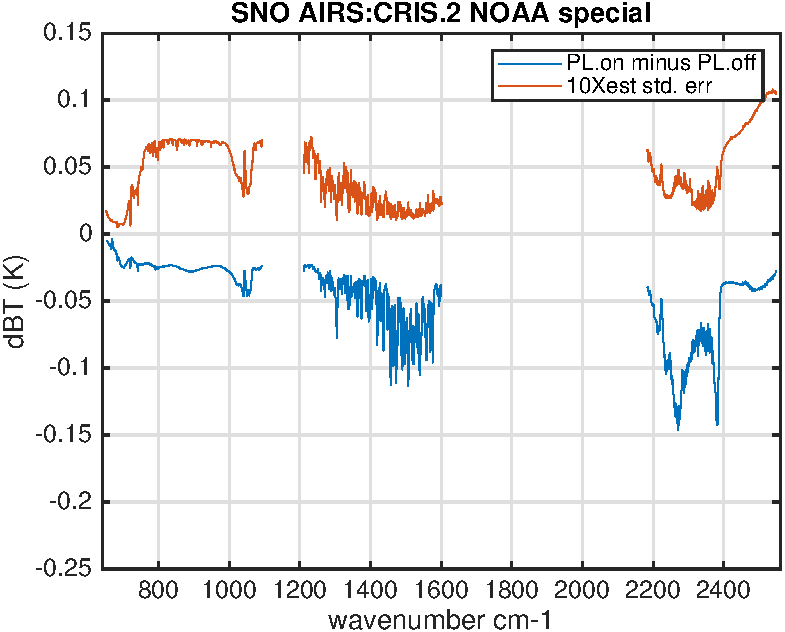
\includegraphics[width=0.75\textwidth]{Figs/sno_airs_cris2_bias_dble_diff_spectrum_polz.pdf}
  \end{center}
   
\end{frame}
% --------------------------------------------------------------------
\begin{frame}
  \frametitle{Impact of the polarization correction on the bias with AIRS}
  \vspace{-0.125in} %\relscale{0.95}
  \begin{itemize}
     \item LW band: 
  \end{itemize}
  
  \begin{center}
    \noindent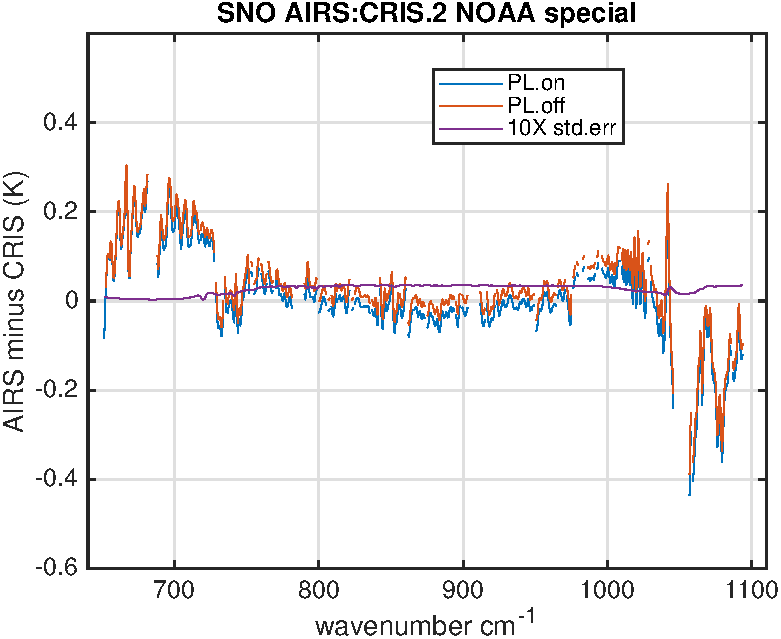
\includegraphics[width=0.75\textwidth]{Figs/sno_airs_cris2_bias_spectrum_polz_lw.pdf}
  \end{center}
   
\end{frame}
% --------------------------------------------------------------------
\begin{frame}
  \frametitle{Impact of the polarization correction on the bias with AIRS}
  \vspace{-0.125in} %\relscale{0.95}
  \begin{itemize}
     \item MW band: 
  \end{itemize}
  
  \begin{center}
    \noindent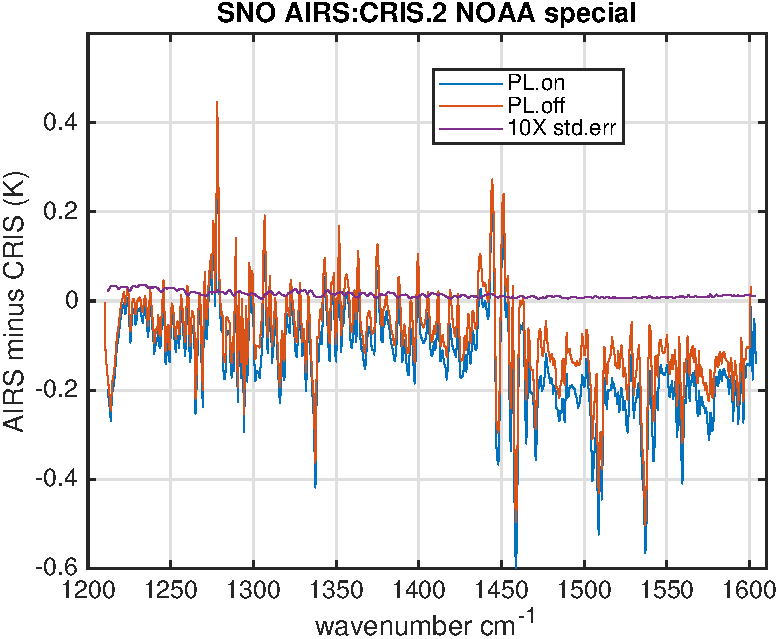
\includegraphics[width=0.75\textwidth]{Figs/sno_airs_cris2_bias_spectrum_polz_mw.pdf}
  \end{center}
   
\end{frame}
% --------------------------------------------------------------------
\begin{frame}
  \frametitle{Impact of the polarization correction on the bias with AIRS}
  \vspace{-0.125in} %\relscale{0.95}
  \begin{itemize}
     \item SW band: 
  \end{itemize}
  
  \begin{center}
    \noindent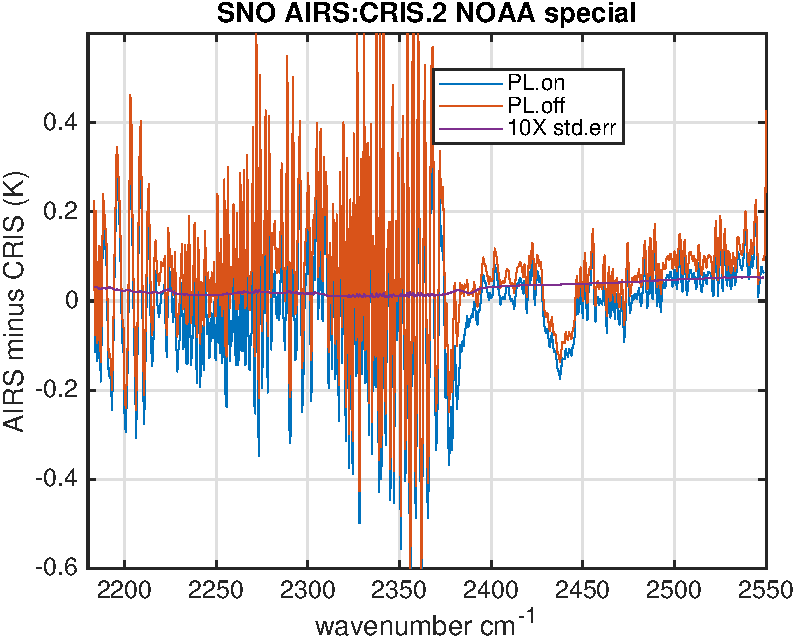
\includegraphics[width=0.75\textwidth]{Figs/sno_airs_cris2_bias_spectrum_polz_sw.pdf}
  \end{center}
   
\end{frame}
% --------------------------------------------------------------------
\begin{frame}
  \frametitle{Discussion}
  \vspace{-0.1 in}
  \begin{itemize}
     \item 
  \end{itemize}

  
\end{frame}

\end{document}

%%%%%%%%%%%%%%%%%%%%%%%%%%%%%%%%%%%%%%%%%%%%%%%%%%%%%%%%%%%%%%%%%%%%%%%%
